In order to test the validity of using neural networks sampled
from molecular dynamics trajectories to generate new trajectories
we train neural networks on systems of copper and silicon atoms
using the Effective Medium Theory and Stillinger-Weber potentials
respectively.
At temperatures which are not too large these potentials describe
atoms in a crystalline structure in equilibrium,
and we test whether the neural network can reproduce the correct potential
energy, forces, radial distribution and mean squared displacement.


\begin{table}[h]
\label{tab:hyperparam}
\caption{Hyperparameters used in fitting.}
\begin{center}
\begin{tabular}{|c c|}
\hline
Hyperparameter & Value \\
\hline \hline
Features & 8 \\
Hidden layers & $(10, 10, 10)$ \\
Activation & Hyperbolic tangent \\
Timesteps & $10^4$ \\
Max epochs & 10000 \\
Optimizer & Adam \\
Initial learning rate & $10^{-3}$ \\
Energy RMSE & $10^{-3}$eV \\
Energy coefficient & 1.0 \\
Force RMSE & $7.5\cdot10^{-2}$eV/Å \\
Force coefficient & 0.04 \\
\hline
\end{tabular}
\end{center}
\end{table}

\subsection{Effective Medium Theory}
The Effective Medium Theory (EMT) potential gives a good description
of the late transition metals in a Face-Centered Cubic (FCC) crystal
lattice, and has a very efficient implementation in ASE,
which makes it ideal for producing large amounts of data.
We will use a rather small system of $4 \times 2^3 = 32$ atoms
for training, since this means a larger amount of labels available
for atoms when we are only using the potential energy.
We train with only the energy for $8 \cdot 10^5$ steps
writing to file every 100 steps and then subsequently
train using both energy and forces for $5 \cdot 10^4$ steps
for a total of 500 configurations. We train on both sets of images
for 2000 steps, where the BFGS optimizer has generally converged.
\par
After the calculator is trained we compare the performance
of the neural network with the EMT potential on a system
of 32 atoms with a temperature of 300 Kelvin for 5000 steps.

\subsection{Stillinger-Weber}
Text.

\begin{figure}[h]
    \centering
    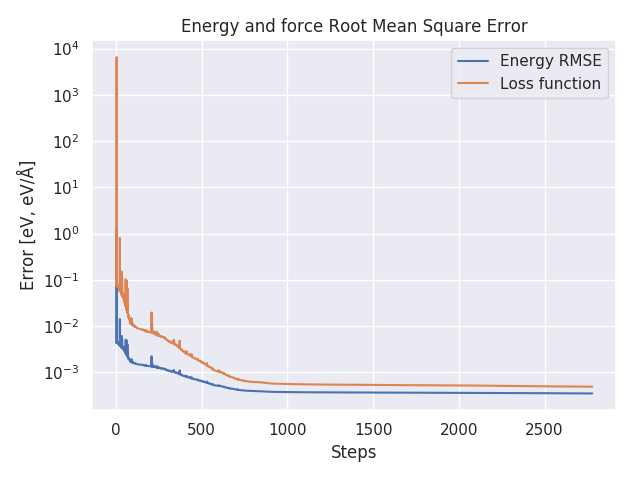
\includegraphics[width=\linewidth]{convergence_stillinger_weber.png}
    \caption{Placeholder}
    \label{fig:msd}
\end{figure}

\begin{figure}[h]
    \centering
    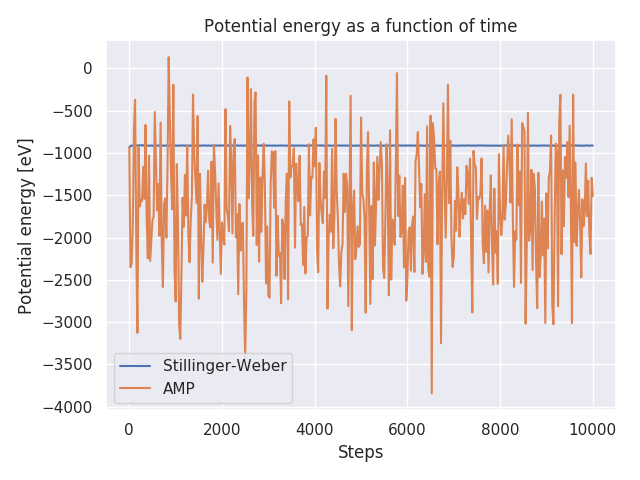
\includegraphics[width=\linewidth]{energy_stillinger_weber.png}
    \caption{Placeholder}
    \label{fig:msd}
\end{figure}

\begin{figure}[h]
    \centering
    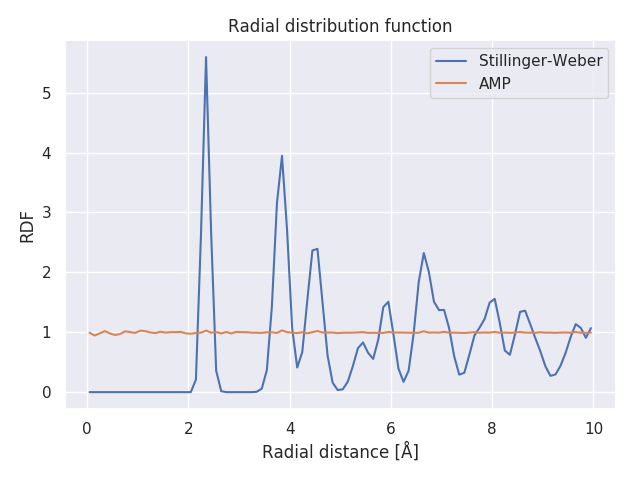
\includegraphics[width=\linewidth]{rdf_stillinger_weber.png}
    \caption{Placeholder}
    \label{fig:msd}
\end{figure}

\begin{figure}[h]
    \centering
    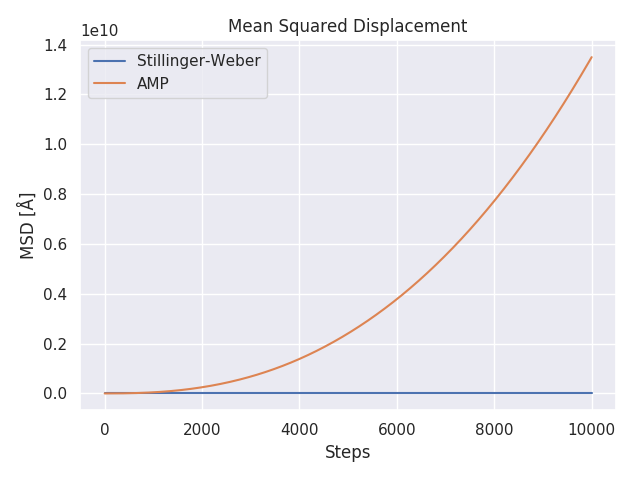
\includegraphics[width=\linewidth]{msd_stillinger_weber.png}
    \caption{Placeholder}
    \label{fig:msd}
\end{figure}
